\documentclass[12pt,a4paper]{article}
\usepackage[lmargin=3cm, tmargin=3cm, rmargin=2cm, bmargin=2cm]{geometry}
\usepackage{sbc-template}
\usepackage{graphicx,url}
\usepackage[utf8]{inputenc}  
\usepackage{ragged2e}
\usepackage{setspace}
\onehalfspacing
\setlength{\parindent}{1.25cm}
\usepackage{indentfirst}
\usepackage{graphicx}
\usepackage{float}
\usepackage{url}
\usepackage[brazil]{babel}
\usepackage{hyperref}
\sloppy

\title{CTP Acolhe}

\author{Isabela C. Silva, Jéssica S. Silva, Kaio Victtor Galvão, Maria Eduarda Lúcio,\\ Matheus S. Portes, Nickolas T. Silva, Werônica A. Melo}

 \address{Instituto Federal de Educação, Ciência e Tecnologia de São Paulo (IFSP)\\
 São Paulo -- SP -- Brasil\\  Curso Técnico em Informática Integrado ao Ensino Médio\\ PDS - Prática para Desenvolvimento de Sistemas}

\begin{document} 

\maketitle

\begin{abstract}
  This document is the result obtained until the preparation of the POC of "CTP Acolhe", a project that aims to improve the contact of the students with the CTP, an IFSP department that offers pedagogical and psychological help to its students. Therefore, the project aims to provide anyone with the help they need in a simpler and more direct way, through a web system that will be responsible for managing consultations with psychologists and organizing studies.

\end{abstract}
     
\begin{resumo} 
  Este documento é o resultado obtido até a elaboração da POC do "CTP Acolhe", um projeto que visa melhorar o contato dos alunos com a CTP. O projeto tem como objetivo possibilitar para os alunos do Instituto Federal do Campus Sâo Paulo, a ajuda que precisam de uma maneira mais simples e direta, através de um sistema web que será responsável por gerenciar os atendimentos com os psicólogos e organização de estudos.
\end{resumo}

\newpage

\listoffigures

\newpage
\begin{description}
        \item \textbf{Lista de siglas e abreviaturas}\\
        \item CTP Cordenadoria Técnico-Pedagógica
        \item DSP Diretoria adjunta Sociopedagógica
        \item IFSP Instituto Federal de Educação, Ciência e Tecnologia de São Paulo
        \item LGPD Lei Geral De Proteção de Dados Pessoais
        \item PDS Prática para Desenvolvimento de Sistemas
        \item POC Prova de Conceito
        \item UI Design de interface de usuário
        \item UX Experiência do usuário
        
\end{description}

\newpage

\tableofcontents

\newpage

\section{Introdução}
\pagestyle{plain}
\pagenumbering{arabic}

O presente documento visa apresentar a \textit{Prova de Conceito (POC)} do projeto de planejamento e execução de um sistema Web que está sendo desenvolvido por meio da disciplina de \textit{PDS (Prática para Desenvolvimento de Sistemas)}, e através dos conhecimentos adquiridos ao longo dos anos de curso Técnico em Informática integrado ao Ensino Médio no IFSP. 

Analisando os requisitos da disciplina, bem como os objetivos da equipe, os integrantes da Lotus pensaram em uma aplicação que pudesse solucionar ou minimizar dificuldades do cotidiano. Assim, após muitas ideias e reflexões, chegaram a um problema presente dentro da Instituição IFSP – Câmpus São Paulo: a falta de conhecimento e dificuldade no acesso a \textit{Coordenadoria Técnico-Pedagógica (CTP)}. Esta opera acolhendo dúvidas e solicitações da comunidade escolar, oferecendo atendimentos individuais e/ou em grupo com orientação e acompanhamento pedagógico e/ou psicológico (na área da Psicologia Escolar), e também disponibiliza orientações técnicas ao corpo discente. 

O acesso à CTP se dá através do e-mail da Coordenadoria, o que torna o processo de contato mais demorado. Ademais, muitos integrantes da instituição não conhecem os serviços oferecidos pela CTP. Sabendo das dificuldades que os alunos enfrentam na vida escolar, e como um setor como a Coordenadoria Técnico-Pedagógica é importante, o projeto CTP Acolhe busca tornar a comunicação e o conhecimento dele mais acessível aos alunos do Instituto Federal do Câmpus São Paulo. Para mais, busca ajudar nos processos internos da CTP, possibilitando qualidade e conforto para os estudantes e funcionários.   

As principais funcionalidades do sistema foram selecionadas e desenvolvidas para serem apresentadas nesta etapa de construção do projeto, a Prova de Conceito, visando demonstrar a viabilidade da aplicação tal qual os processos específicos do negócio. 

Assim, diante da dificuldade apresentada em relação ao conhecimento e acesso a Coordenadoria Técnico-Pedagógica do IFSP, a Prova de Conceito do projeto CTP Acolhe apresenta as funcionalidades iniciais da aplicação e o que foi utilizado para que seu desenvolvimento fosse possível.

\subsection{Justificativa}

A equipe realizou uma pesquisa que deu iniciativa ao projeto. Esta foi realizada por meio eletrônico, através de um formulário com questões relacionadas à proposta inicial. Durante o período de divulgação da pesquisa, que se passou entre os dias 16 de março de 2023 e 11 de abril do mesmo ano, foi obtido um total de 45 respostas, efetuadas por somente alunos matriculados no Instituto Federal de São Paulo, sendo 21 do Curso Técnico de Informática Integrado ao Ensino Médio, 7 do Curso Técnico de Mecânica Integrado ao Ensino Médio, 5 do Curso Técnico de Desenvolvimento de Sistemas Integrado ao Ensino Médio, 2 do Curso Técnico de Eletrônica Integrado ao Ensino Médio, 1 da Licenciatura em Ciências Biológicas, 7 da Licenciatura em Letras, e 2 que não identificaram o curso. Os alunos atenderam um total de 8 perguntas principais. 

Por intermédio dessa pesquisa, é perceptível e afirmável que 82,2\% dos entrevistados já sentiram dificuldades no que diz respeito à organização de seus estudos (Figura~\ref{fig01}).

\begin{figure}[H]
    \centering
    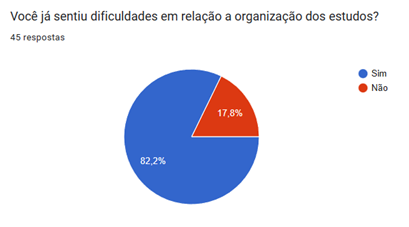
\includegraphics[width=12cm]{img1.png}
    \caption{Discentes que já sentiram dificuldades em relação à organização de seus estudos}
    \label{fig01}
\end{figure}

Ao ser questionado, foi possível concluir que a quantidade de entrevistados que, em algum momento de sua experiência estudantil, já sentiram que precisavam de ajuda psicológica para lidar com a situação de pressão estudantil no IFSP foi maior do que a quantidade de alunos que não sentiram a mesma necessidade (Figura~\ref{fig02}). 

\begin{figure}[H]
    \centering
    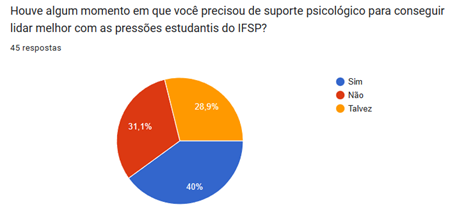
\includegraphics[width=14cm]{img2.png}
    \caption{Necessidade de suporte psicológico para lidar com as pressões estudantis no IFSP}
    \label{fig02}
\end{figure}

Apesar de majoritariamente parte dos estudantes demonstrarem indiretamente carência de ferramentas proporcionadas por serviços assegurados pela \textit{Coordenadoria Técnico-Pedagógica (CTP)}, a grande maioria, isto é, 73,3\% dos discentes, nunca tentaram entrar em contato com a CTP (Figura~\ref{fig03}).

\begin{figure}[H]
    \centering
    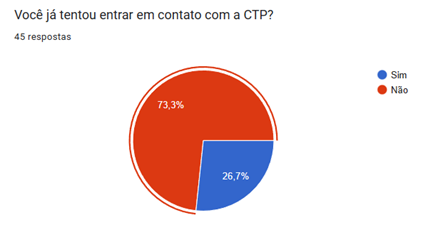
\includegraphics[width=12cm]{img3.png}
    \caption{Entrevistados que tentaram entrar em contato com a CTP}
    \label{fig03}
\end{figure}

O baixo índice de interesse no sentido de estabelecer contato com a \textit{Coordenadoria
Técnico-Pedagógica (CTP)} pode ser explicado pela falta de divulgação da atuação do setor Sociopedagógico do Câmpus, bem como pela dificuldade encontrada por parte dos alunos na busca pelo serviço disponibilizado pela CTP.

Após indagar dos estudantes o que eles estimavam de uma plataforma que tivesse o intuito de facilitar o contato entre o aluno e a CTP, obteve-se que 86,7\% das respostas julgaram como uma plataforma necessária, enquanto apenas uma resposta foi contrária a ideia (Figura~\ref{fig04}).

\begin{figure}[H]
    \centering
     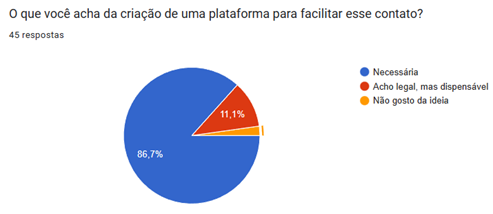
\includegraphics[width=15cm]{img4.png}
    \caption{Entrevistados que consideram como necessária a criação da plataforma}
    \label{fig04}
\end{figure}

Possuindo e analisando esses dados, faz-se importante a criação de um sistema (aplicação web) que facilite a comunicação entre o estudante do IFSP e a \textit{Coordenadoria Técnico- Pedagógica (CTP)}, para que os alunos que apresentam alguma necessidade e sentem dificuldade de estabelecer contato ou entender o funcionamento do setor sejam auxiliados; além de organizar a demanda que chega para a CTP em função dos processos e incidentes.

 Ademais, em ciência após diálogo com a \textit{Coordenadoria Técnico-Pedagógica (CTP)}, atualmente não chegam somente inquisições acerca de acompanhamentos psicológicos, mas também dúvidas gerais que geralmente são tratadas por outro setor e de outra forma, uma vez que a CTP integra também a \textit{Diretoria adjunta Sociopedagógica (DSP)}. Assim, igualmente se faz necessário, pois é capaz de organizar os processos que chegam para a \textit{Coordenadoria Técnico-Pedagógica (CTP)}, minando qualquer tipo de atraso ou confusão no momento de atender as exigências e estabelecer ordem de importância para tais. 

\subsection{Objetivo}

O projeto CTP Acolhe tem como objetivo tornar mais fácil a comunicação direta entre os alunos e a \textit{
CTP (Coordenadoria Técnico-Pedagógica)} do IFSP, centralizando esses incidentes, ao mesmo tempo que divulga o seu apoio pedagógico e psicológico aos estudantes. 

Além disso, por meio de perguntas e respostas, a equipe fará uma coleta de informações iniciais importantes para caracterizar cada incidente, com o intuito de melhorar a organização desses incidentes por prioridades, de acordo com requisitos que estão sendo discutidos com a CTP durante o desenvolvimento do projeto. 

Os integrantes da Lotus também buscam passar confiança e segurança aos alunos que buscarem ajuda através do CTP Acolhe, pois, ainda que seja normal precisar de ajuda, muitos alunos podem sentir medo de serem expostos ou se sentirem vulneráveis ao entrar em contato com a Coordenadoria Técnico-Pedagógica em busca de auxílio. 

\section{Designe}
\subsection{Logo do Sistema/Aplicação}
Com o escopo do projeto definido, a próxima etapa da equipe foi estipular uma marca que caracterizasse  a aplicação. 
Dessa forma, foi definida a seguinte logo para o sistema CTP Acolhe: (Figura~\ref{ft01}).

\begin{figure}[H]
    \centering
     
\includegraphics[width=12cm]{ft.png}
    \caption{Logo}
    \label{ft01}
\end{figure}

Logomarca essa que foi feita utilizando a ferramenta do FIGMA e de um banco de imagens gratuito, o FreePik. Com a Logo, já foram definidas as cores principais do sistema e a tipografia de fontes – auxiliando, assim, o desenvolvimento das etapas posteriores do projeto, como o desenvolvimento da UI e da UX \cite{aela}.

\subsection{UI/UX Designe}
UI Design tem com enfoque a interface de um determinado sistema; já a UX tem como objetivo a experiência final do usuário, envolvendo todo o caminho que ele faz na aplicação até encontrar seu objetivo (BrainBlog).
Assim, na próxima etapa do desenvolvimento do design da aplicação, o pensamento foi de que – desde o momento que o usuário entrasse pela primeira vez, até o momento que saísse – a aplicação propusesse uma experiência intuitiva enquanto estivesse sendo utilizada. E, por ser um sistema que é voltado para os estudantes e a Coordenadoria Técnico Pedagógica, a acessibilidade e o fácil acesso foram priorizados \cite{aela}.

\section{Análise de Requisitos}
A análise de requisitos visa identificar e definir as necessidades que o usuário espera sanar com o sistema que será desenvolvido, além de permitir explicitar as funcionalidades, permissões e as restrições do projeto. Desse modo, foi realizado pela equipe o levantamento dos Requisitos Não Funcionais (RNF), Requisitos Funcionais (RF) e as Regras de Negócio (RN). \cite{vverner, mestres, artigoo} 

\subsection{Requisitos Não Funcionais (RNF)}
Os Requisitos Não Funcionais são aqueles que tratam dos atributos de qualidade que o sistema deve possuir como um todo, e não das funcionalidades específicas que são oferecidas por esse sistema. Visto a importância desse levantamento, foi realizado na (Figura~\ref{fig05}), listando os Requisitos Não Funcionais para o projeto CTP Acolhe: (Figura~\ref{fig05}). \cite{artigo, blog, codificar}

\newpage 

\begin{figure}[H]
    \centering
     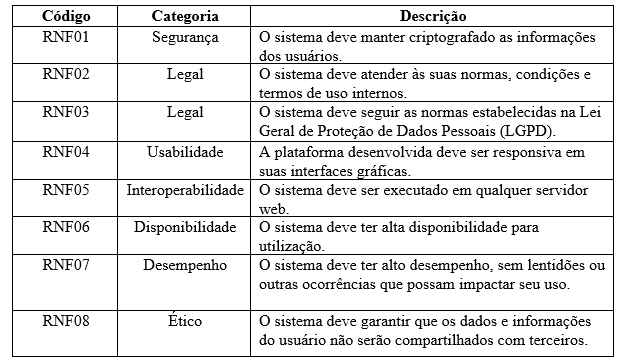
\includegraphics[width=15cm]{img5.png}
    \caption{Descrição de requisitos não funcionais}
    \label{fig05}
\end{figure}

\subsection{Requisitos Funcionais (RF)}
Os Requisitos Funcionais são aqueles que especificam as funções e comportamentos que o sistema deverá seguir para atender às expectativas do usuário. É ideal que se defina o nível de prioridade para cada um desses requisitos a fim de definir sua importância e o esforço necessário para sua realização. Portanto, visando as principais funcionalidades do sistema, a equipe classificou os Requisitos Funcionais \cite{codificar}, em Alta, Média e Baixa prioridade: (Figura~\ref{o6})

\newpage

\begin{figure}[H]
    \centering
     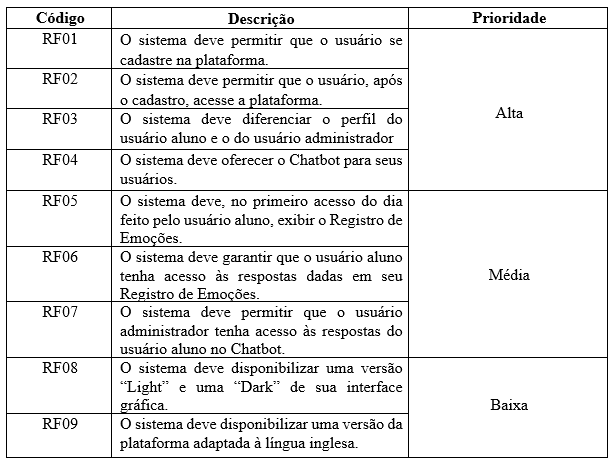
\includegraphics[width=15cm]{img6.png}
    \caption{Descrição de requisitos funcionais}
    \label{o6}
\end{figure}

\subsection{Regras de Negócio (RN)}
As regras de negócio são um conjunto de declarações explícitas que definem como um negócio opera e quais são suas especificações. Essas declarações descrevem políticas, procedimentos, valores e restrições do negócio.

Segundo Dallavalle e Cazarini (2000), as Regras de Negócio são fundamentais pois afetam diretamente os requisitos funcionais do sistema; uma vez que, são regras do domínio de aplicação que devem ser tratadas no desenvolvimento.
Portanto, depreende-se que devem ser levantadas e documentadas de forma clara e objetiva, de modo a garantir com que todos compreendam as especificações do negócio. \cite{artigoo}

A documentação das regras de negócio envolve várias formas de representação e a escolha da melhor forma de fazê-la depende da complexidade do negócio e das necessidades do planejamento e dos stakeholders. Nesse sentido, para definir as regras de negócio, foi realizado a (Figura~\ref{p1}) que dispõe as Regras de Negócio do projeto CTP Acolhe. \cite{artigoo}

\newpage

\begin{figure}[H]
    \centering
     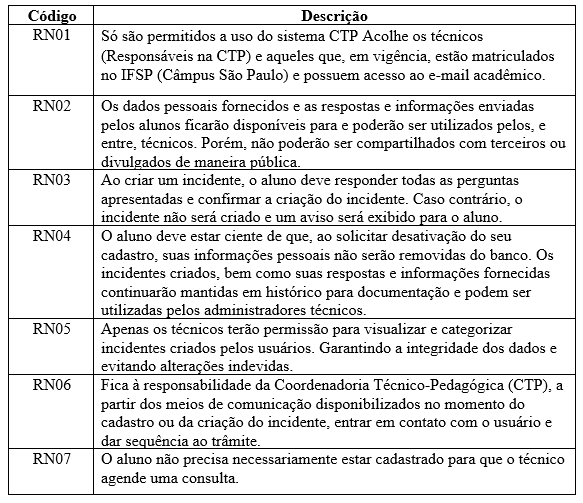
\includegraphics[width=15cm]{img8.png}
    \caption{Regras de Negócio}
    \label{p1}
\end{figure}

\section{Métodos de Gestão}
Para garantir que a organização do projeto, a definição de tarefas, os prazos de entrega e o desenvolvimento do sistema ocorram de forma eficaz, saudável e ágil para todos os membros da equipe, foram adotada metodologias ágeis que auxiliam a produtividade e a entrega de bons resultados no projeto.

Dentre as diversas metodologias ágeis, a equipe optou por selecionar o modelo Scrum, pois é voltado para a gestão e planejamento de projetos de Software e se enquadra nas necessidades que o projeto demanda. No entanto, houve adaptações nos padrões dessa metodologia para que sua aplicação fosse viável:

\begin{itemize}
    \item \textbf{Sprint:} Ciclos de atividades que foram adaptadas para durarem até duas semanas, devido às entregas frequentes que são exigidas pela disciplina;\cite{roberto}
    \item \textbf{Time-Boxed:} Tempo estipulado para que as atividades da Sprint sejam cumpridas, e que pode ser adaptado conforme a disponibilidade dos membros da equipe e por sua data de entrega;\cite{roberto}
    \item \textbf{Planejamento de Sprint:} Reuniões realizadas no início de cada ciclo para priorizar, definir como será feito e destituir as tarefas entre a equipe. Tais reuniões ocorrerão no dia seguinte ao fim da Sprint anterior e durarão cerca de 2 horas; \cite{roberto}
    \item \textbf{Reuniões diárias:} Não sendo possível realizar reuniões diárias de forma síncrona, a equipe optou por, diariamente, manter a comunicação sobre o desenvolvimento de cada tarefa de forma assíncrona, através dos canais de comunicação como WhatsApp ou Discord; \cite{roberto}
    \item \textbf{Revisão da Sprint:} A revisão da Sprint ocorrerá durante todo o seu desenvolvimento, seja nas aulas da disciplina de PDS, em atendimento aos alunos ou nas reuniões com a CTP, para que, assim, haja um feedback mais rápido sobre as melhorias do que está sendo desenvolvido; \cite{roberto}
    \item \textbf{Retrospectiva da Sprint:} Reunião feita no fim de cada Sprint, com duração de, aproximadamente, 2 horas e que aponta as dificuldades e ajustes encontrados na realização desse ciclo para que, dessa forma, a produtividade seja melhor na próxima Sprint. \cite{roberto}
\end{itemize}

Além da utilização do \textit{Scrum}, o quadro \textit{Kanban} foi escolhido pela equipe para a organização visual das \textit{Sprints}. O quadro em questão apresenta 5 colunas, que dispõem visualmente o estágio de cada tarefa, sendo elas “planejamento”, “a fazer”, “em andamento”, “revisão” e “concluído”. Além disso, cada tarefa possui uma data estipulada para entrega e também é classificada por ordem de prioridade, podendo ser “alta”, representada pela cor vermelha, “média”, representada pela cor amarela, ou “baixa”, representada pela cor verde. \cite{asana}

O quadro \textit{Kanban} foi desenvolvido na plataforma \textit{Trello}, permitindo que o mesmo seja compartilhado entre todos os membros da equipe e que seja acessado de qualquer lugar, para que todos possam fazer ajustes e ter total transparência sobre os itens desenvolvidos (Figura~\ref{l01}).

\begin{figure}[H]
    \centering
     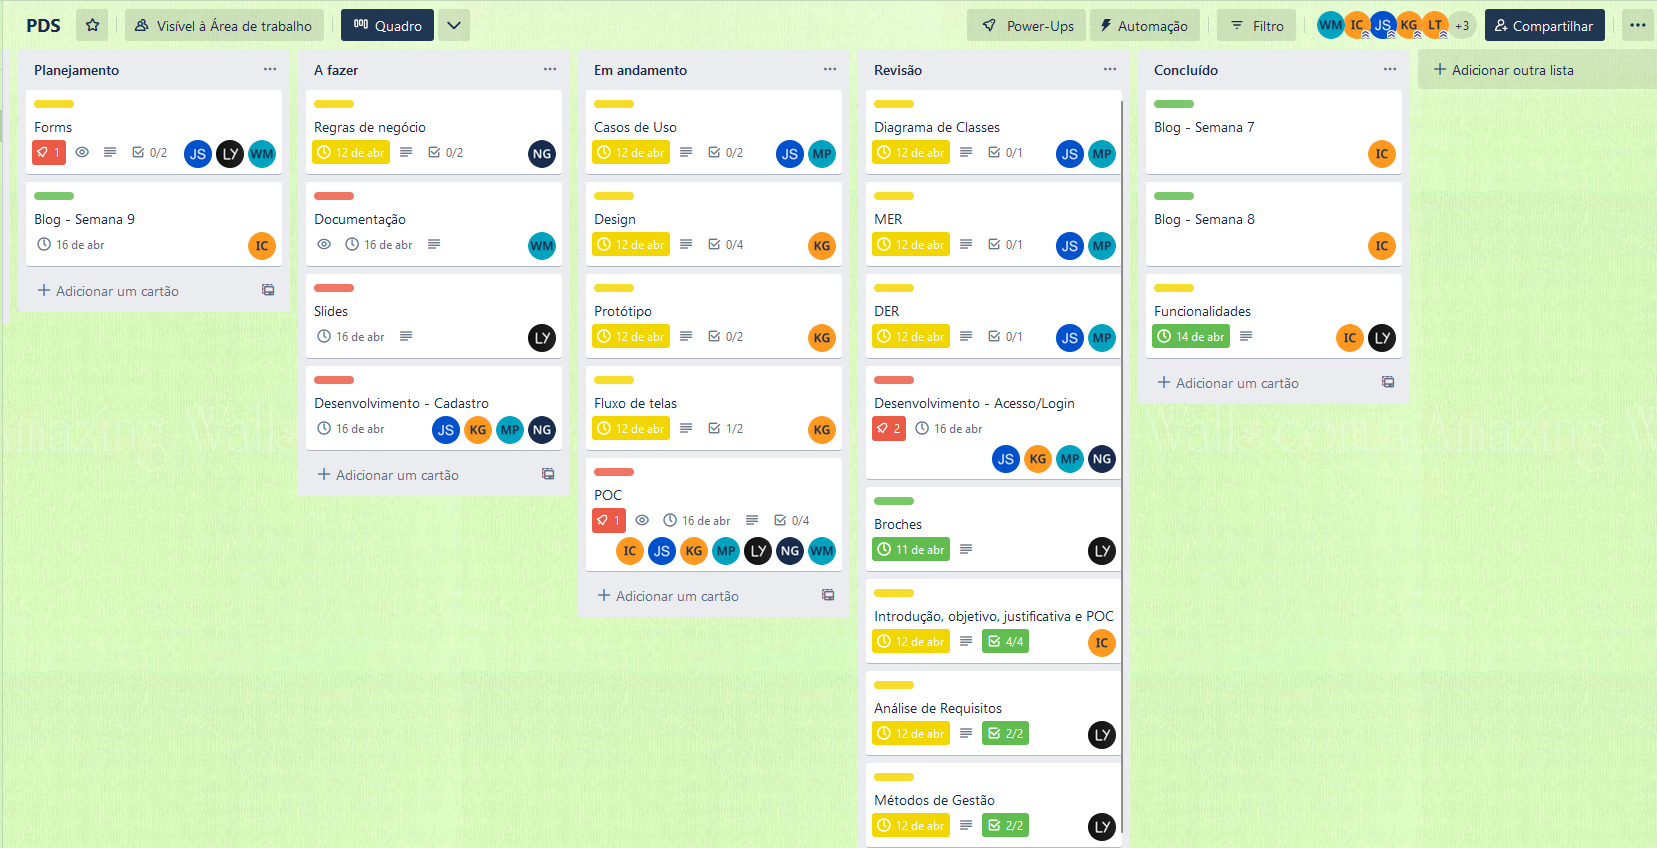
\includegraphics[width=15cm]{img7.png}
    \caption{Quadro de desenvolvimento de tarefas}
    \label{l01}
\end{figure}

\newpage

\section{Modelagem}
\subsection{Diagrma de Casos de Uso}
\begin{figure}[H]
    \centering
     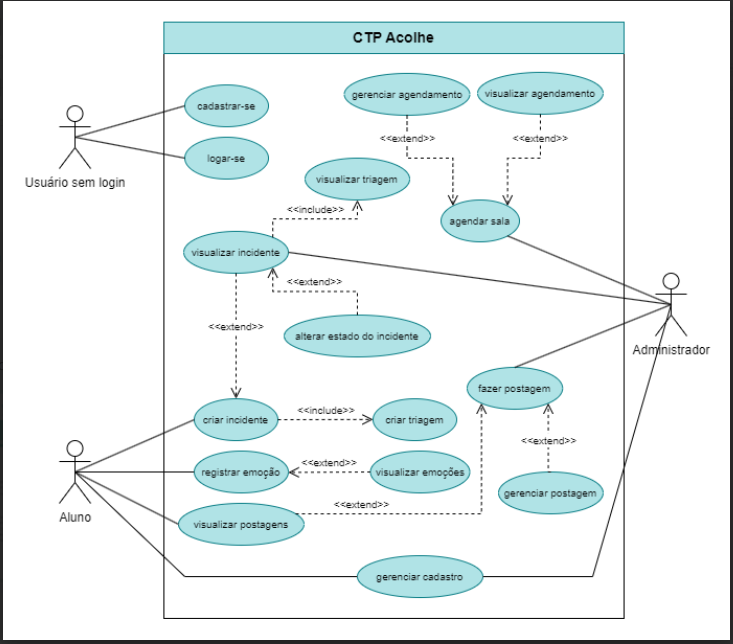
\includegraphics[width=15cm]{casouso.png}
     \caption{Caso de Uso}
     \label{casouso}
\end{figure}

\newpage

\subsection{Diagrma de classes}
\begin{figure}[H]
    \centering
     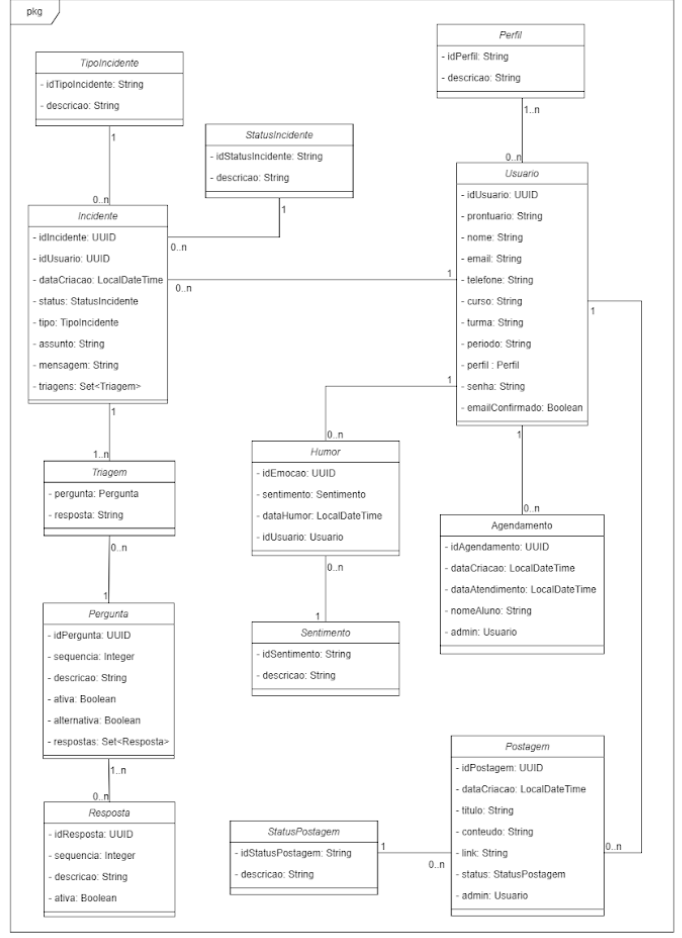
\includegraphics[width=15cm]{diagram.png}
    \caption{Diagrama de classe}
    \label{dia}
\end{figure}

\newpage

\subsection{Diagrama Entidade Relacionamento (DER)}
\begin{figure}[H]
    \centering
     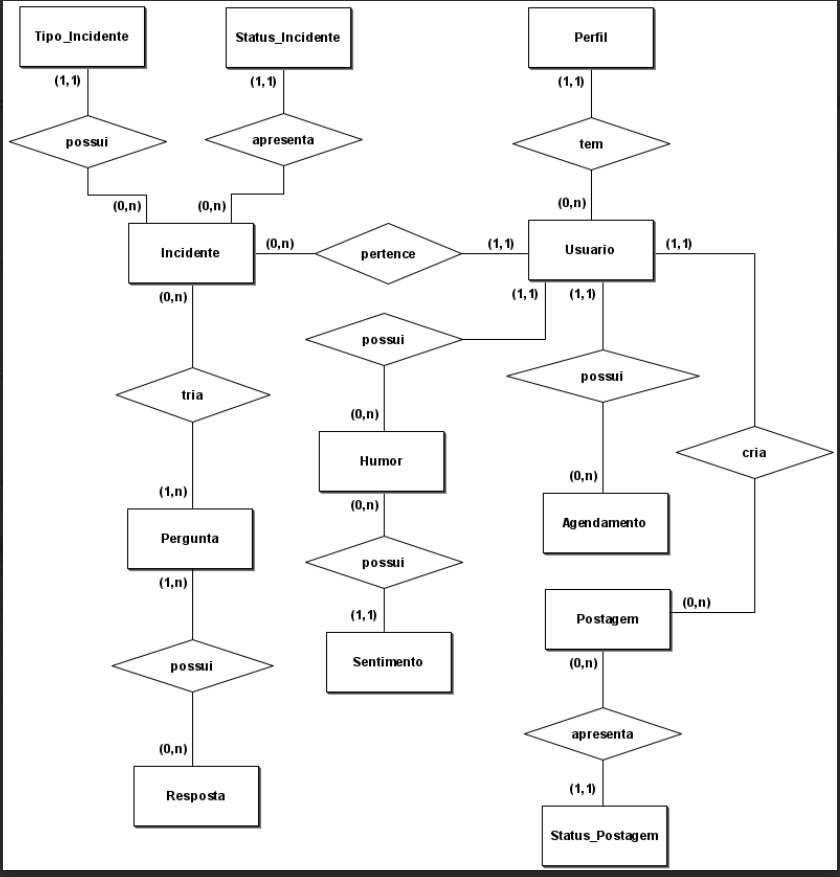
\includegraphics[width=15cm]{der.png}
    \caption{Diagrama Entidade Relacionamento}
    \label{der}
\end{figure}

\newpage

\subsection{Diagrama de Tabelas Relacionais}
\begin{figure}[H]
    \centering
     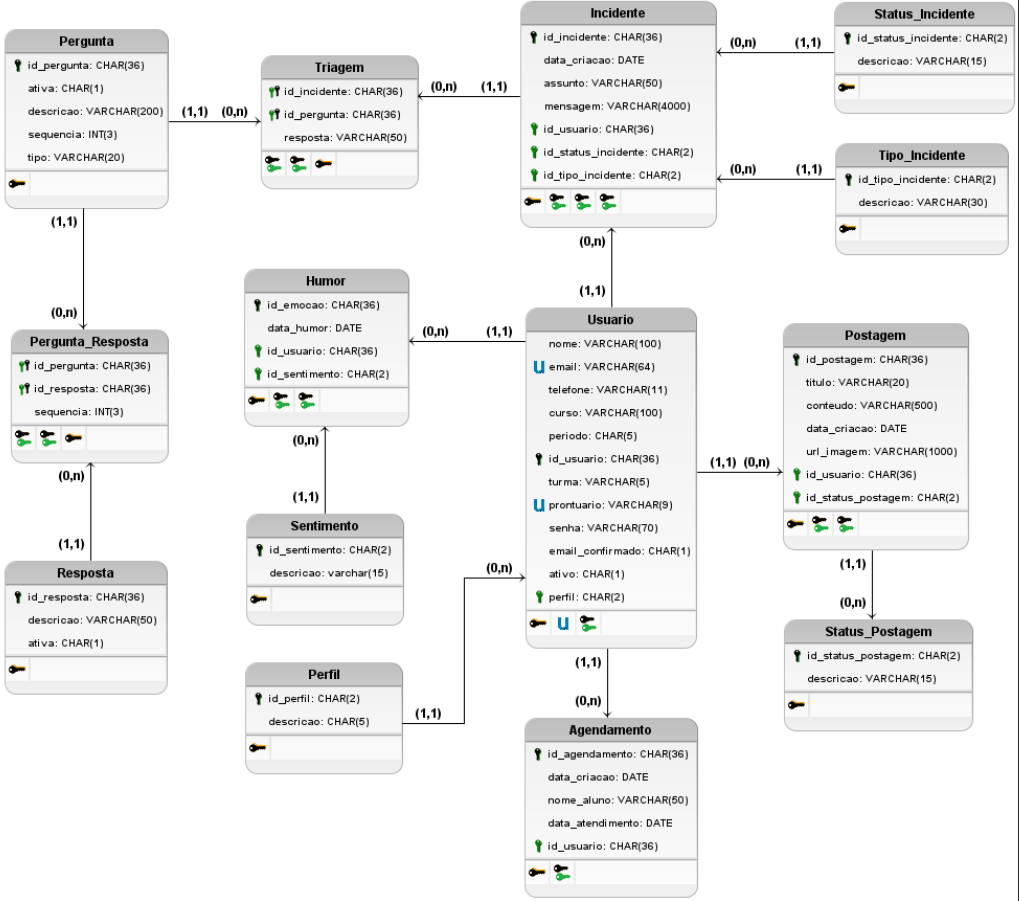
\includegraphics[width=15cm]{mer.png}
    \caption{Diagrama de Tabelas Relacionais}
    \label{mer}
\end{figure}

\section{Prova de Conceito}
O uso da Prova de Conceito possibilita a percepção e análise de uma aplicação com mais clareza, apresentado os riscos e a viabilidade da implementação. Através da realização da POC, é possível colocar em prática as ideias que, até então, sáo apenas teorias, testando funcionalidades e observando se o projeto cumpre com aquilo que se propõe a fazer. 

O desenvolvimento funcionalidades principais de um projeto web através da POC coloca a ideia geral em enquadramento, o que permite que a equipe faça uma análise mais completa de todo o projeto e suas tecnologias, e realize uma estrutura melhor para as demais ideias e funcionalidades. 

Para a realização de uma Prova de Conceito, existem alguns pontos que precisam ser levados em consideração. Em primeiro lugar, é preciso pensar qual é o objetivo dela, o que se pretende alcançar. Em segundo, é preciso pensar no que será testado, quais são as funcionalidades. Além disso, é importante levar em consideração o prazo e o tempo disponível para a realização da POC. Ademais, se faz fundamental analisar os recursos e a equipe. Tendo as respostas dessas questões em mente, é possível produzir a Prova de Conceito \cite{gaspar} \cite{supero}.

\subsection{Prova de Conceito: CTP Acolhe}
A POC do Projeto CTP Acolhe, é formada por duas funcionalidades iniciais da aplicação, sendo elas: o cadastro na plataforma e o acesso do usuário. 

O \textbf{cadastro} pede ao usuário algumas informações, sendo elas: nome, e-mail, curso, período, turma, telefone, senha e confirmação de senha. Essas informações variam de acordo com o tipo de usuário, que pode ser do tipo aluno ou administrador — identificável pelo domínio do e-mail "@aluno.ifsp.edu.br" ou "@ifsp.edu.br".

O \textbf{acesso}, é dividido em dois tipos de usuários: do tipo aluno e do tipo administrador. Para realizar o acesso, é preciso fornecer o e-mail e senha.  

\newpage

\section{Referências}
{\bibliographystyle{plain}}
%\bibliographystyle{abntex2-alf}
\bibliography{sbc-template}

\newpage

\section{Glossário}
\begin{center}
\justifying
    Chatbot 
        Software capaz de manter uma conversa com um usuário humano em linguagem informal. 
\end{center}

\begin{center}
\justifying
    CTP Acolhe 
        Nome dado ao projeto e sistema. 
\end{center}

\begin{center}
\justifying
    Dark
        Esquema de cores mais escuras para a interface. 
\end{center}

\begin{center}
\justifying
    IFSP
        Instituto Federal de Educação, Ciência e Tecnologia de São Paulo. 
\end{center}

\begin{center}
\justifying
    Light
        Esquemas de cores mais claras para a interface.
\end{center}

\begin{center}
\justifying
    RF
        Requisitos Funcionais.
\end{center}

\begin{center}
\justifying
    RNF 
        Requisitos Não Funcionais. 
\end{center}

\begin{center}
\justifying
    RN 
        Regras de Negócio. 
\end{center}

\begin{center}
\justifying
    Servidor Web
        É um sistema de computador capaz de processar solicitações via htpp. 
\end{center}

\begin{center}
\justifying
    Scrum 
        É uma estrutura para gerenciamento de projetos. 
\end{center}

\begin{center}
\justifying
    Sprint
        Cada um dos períodos utilizados para a conclusão de uma parte do projeto. 
\end{center}

\begin{center}
\justifying
    Stakeholders 
        Pessoas, grupos ou organizações que possuem interesse ou podem ser afetados pelas atividades de uma organização. 
\end{center}

\begin{center}
\justifying
    Time-Boxed 
        Tempo de duração para realizar uma determinada tarefa. 
\end{center}

\begin{center}
\justifying
    Trello 
        Ferramenta de Gestão de Projetos. 
\end{center}

\begin{center}
\justifying
    Kanban Método 
        popular de gestão de fluxo de trabalho.
\end{center}
         
\newpage

\section{Apêndices}
\subsection{Apêndice A - Pesquisa de campo}

\begin{figure}[H]
    \centering
     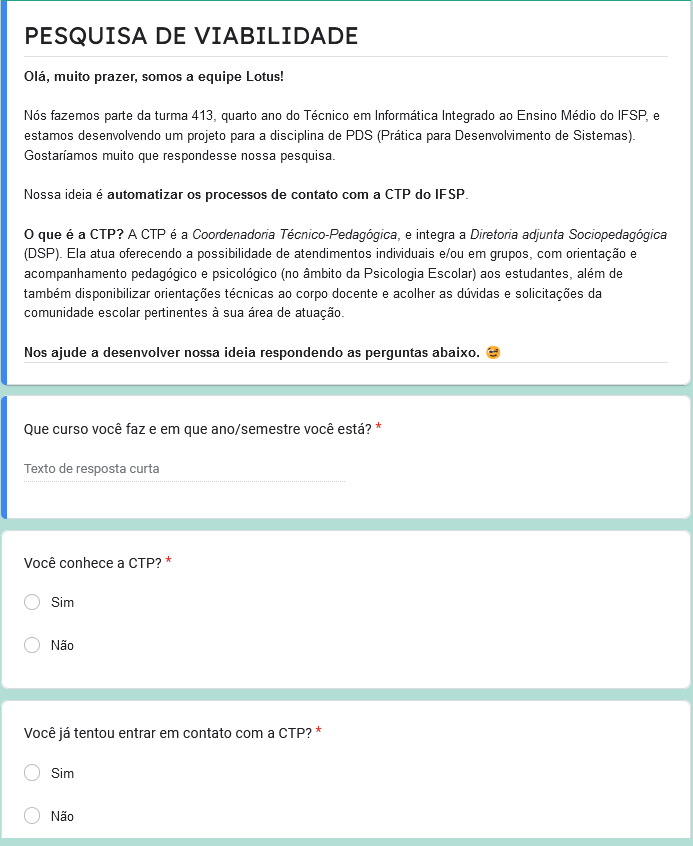
\includegraphics[width=15cm]{foto1.png}
\end{figure}

\newpage

\begin{figure}[H]
    \centering
     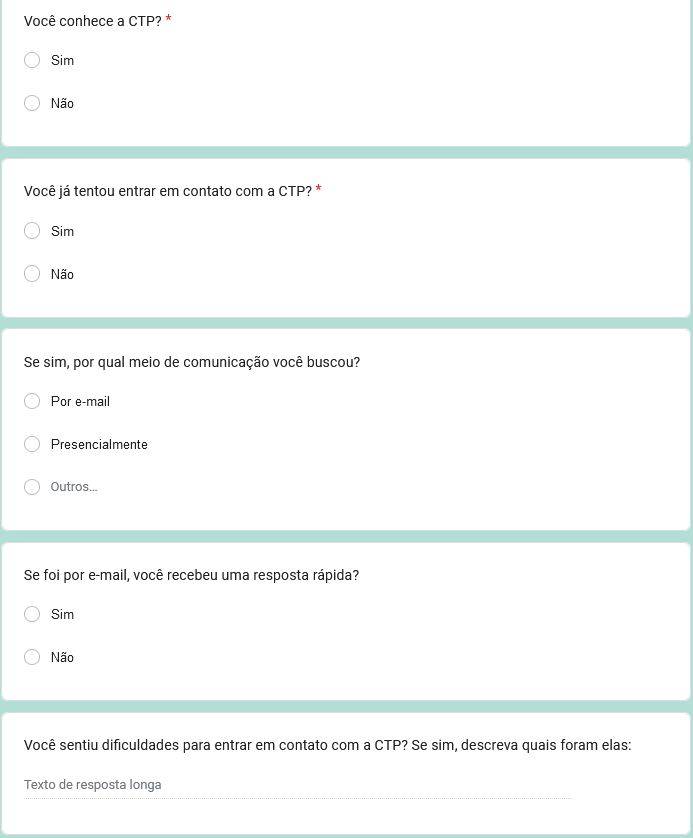
\includegraphics[width=15cm]{foto2.png}
\end{figure}

\begin{figure}[H]
    \centering
     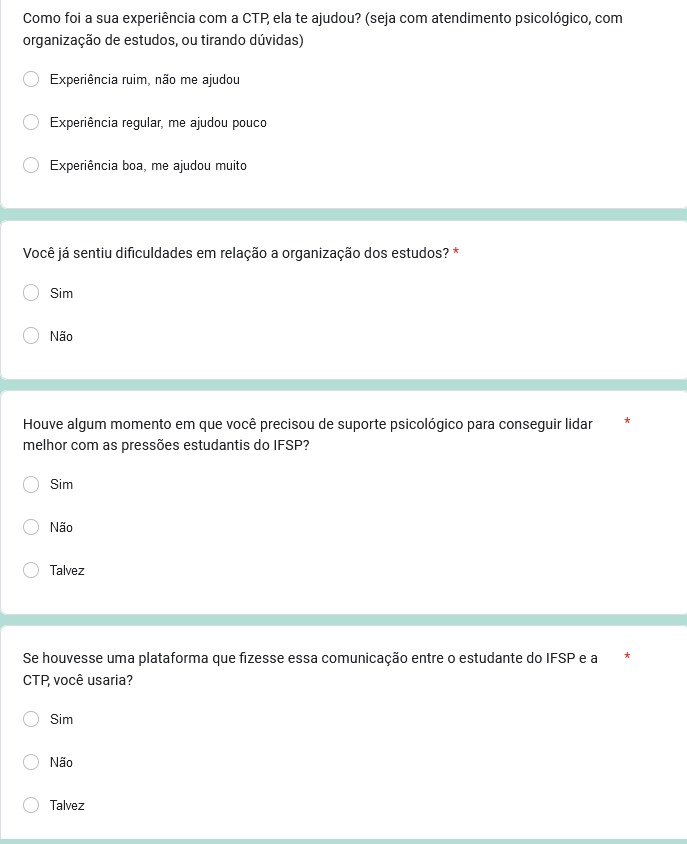
\includegraphics[width=15cm]{foto3.png}
\end{figure}

\begin{figure}[H]
    \centering
     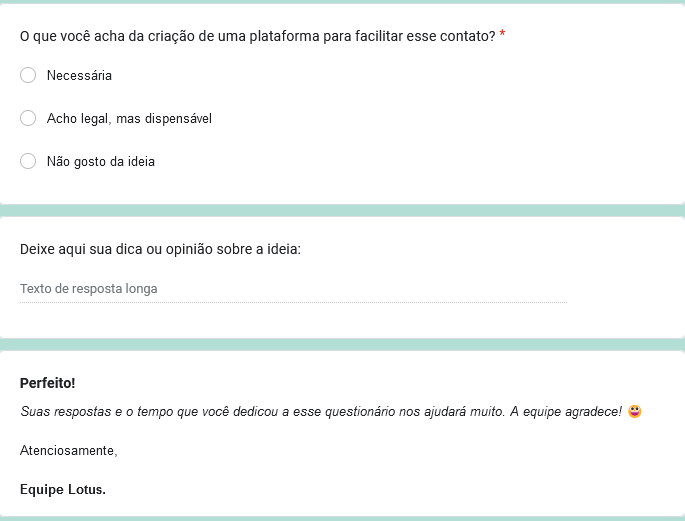
\includegraphics[width=15cm]{foto4.png}
     \caption{Pesquisa de campo}
     \label{fig06}
\end{figure}

\newpage

\subsection{Apêndice B  - Atas de reuniões}
\begin{figure}[H]
    \centering
     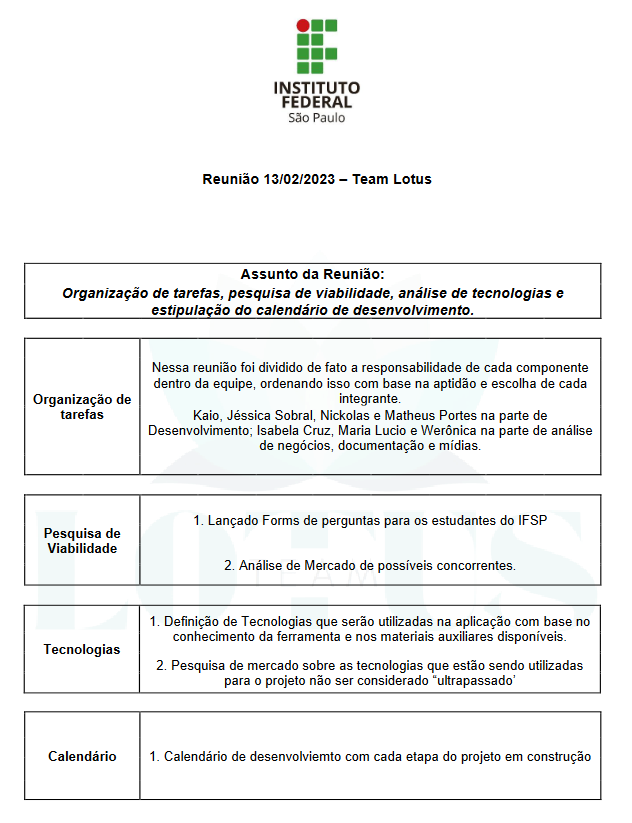
\includegraphics[width=15cm]{ilus1.png}
     \caption{Primeira reunião}
     \label{fig07}
\end{figure}

\begin{figure}[H]
    \centering
     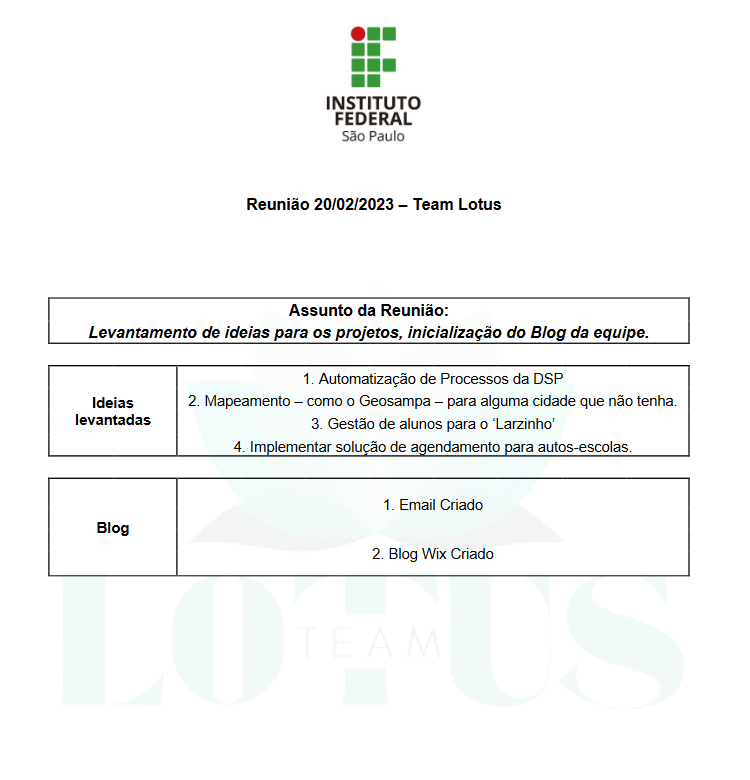
\includegraphics[width=15cm]{ilus2.png}
     \caption{Segunda reunião}
     \label{fig08}
\end{figure}

\begin{figure}[H]
    \centering
     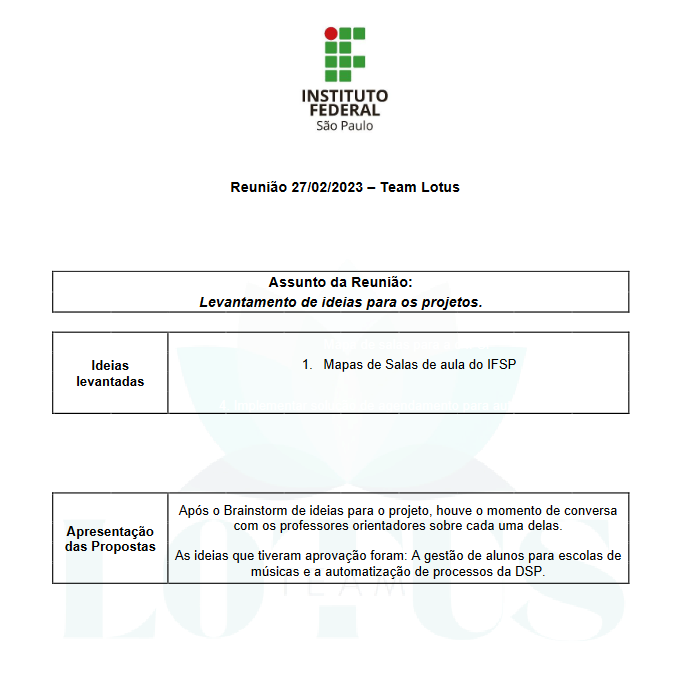
\includegraphics[width=15cm]{ilus3.png}
     \caption{Terceira reunião}
     \label{fig09}
\end{figure}

\begin{figure}[H]
    \centering
     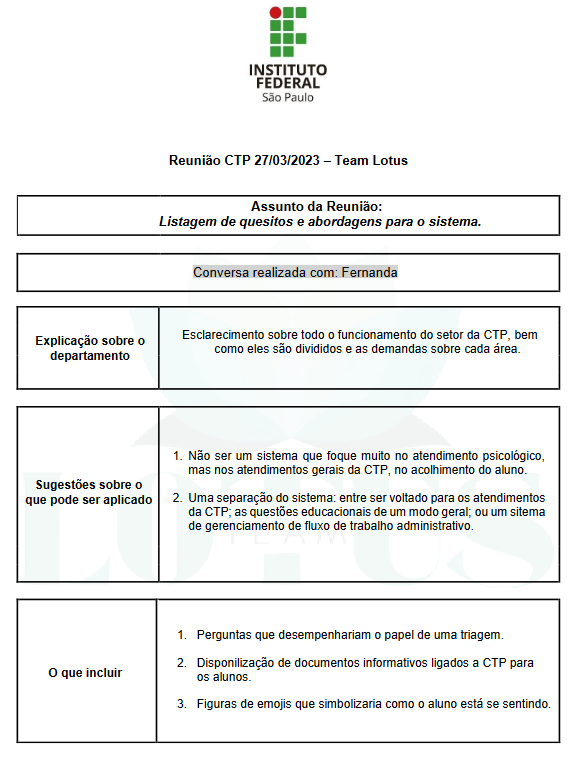
\includegraphics[width=15cm]{ilus4.png}
     \caption{Quarta reunião}
     \label{fig}
\end{figure}

\newpage

\subsection{Apêndice D - Protótipo e Fluxo de Telas}
Em primeira instância, o usuário irá acessar o sistema e será exibido para ele uma Land-Page de apresentação do sistema, juntamente de duas opções: acessar e cadastrar.

\begin{figure}[H]
    \centering
     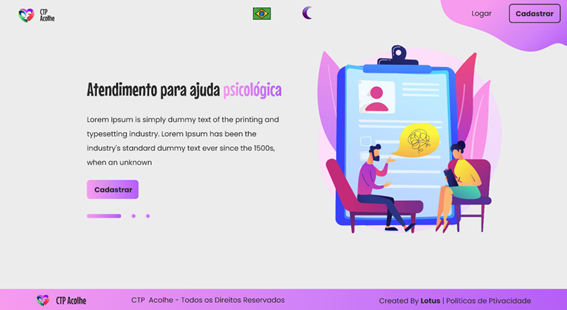
\includegraphics[width=15cm]{prot.png}
     \caption{Homepage}
\end{figure}

Há também a opção do usuário mudar a configuração de linguagem para inglês ou mudar o tema de light para dark.

\begin{itemize}
    \item \textbf{Mudança de Linguagem}
        \begin{figure}[H]
            \centering
            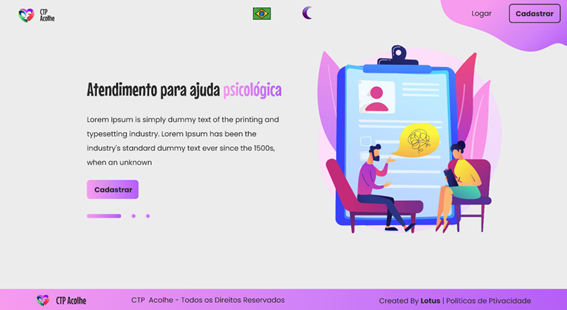
\includegraphics[width=15cm]{prot.png}
            \caption{Homepage mudança de linguagem}
        \end{figure}
    \item \textbf{Mudança de Tema}
        \begin{figure}[H]
            \centering
            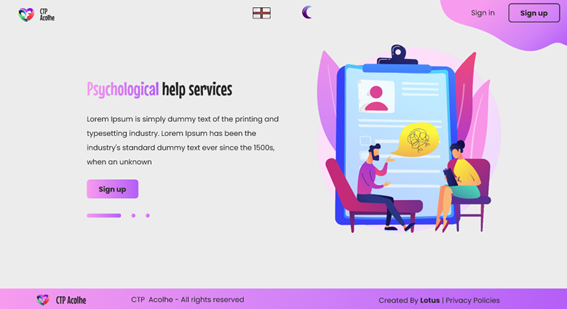
\includegraphics[width=15cm]{prot2.png}
            \caption{Homepage mudança de tem}
        \end{figure}
    \item \textbf{Land Page Slider}
        \begin{figure}[H]
            \centering
            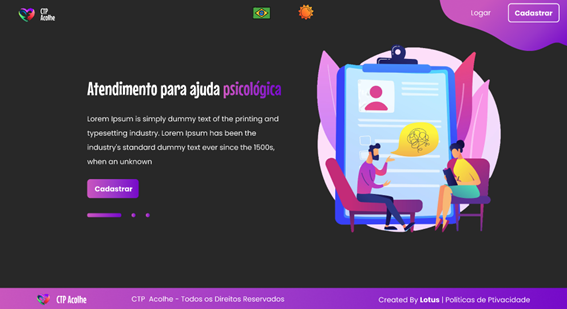
\includegraphics[width=15cm]{prot3.png}
            \caption{Homepage slider}
        \end{figure}
        \begin{figure}[H]
            \centering
            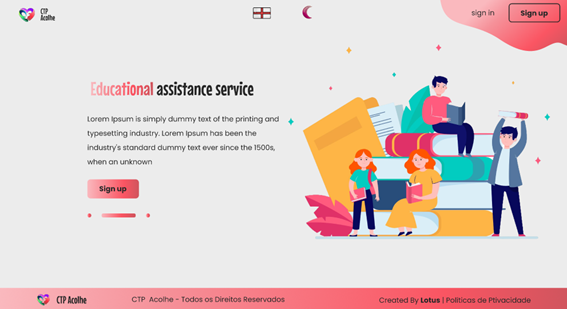
\includegraphics[width=15cm]{prot4.png}
            \caption{Homepage slider}
        \end{figure}
        \begin{figure}[H]
            \centering
            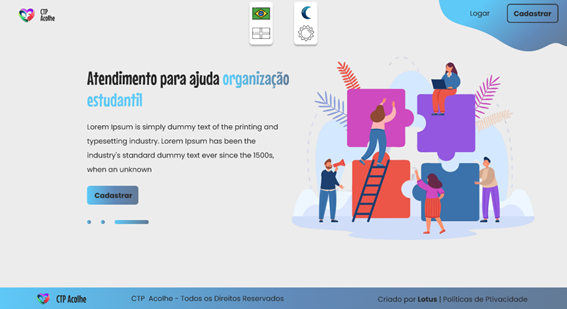
\includegraphics[width=15cm]{prot5.png}
            \caption{Homepage slider}
        \end{figure}
     \newpage
    \item \textbf{Login} \\ \\
    Caso o usuário já tenha uma conta no sistema, ele poderá clicar para fazer o login e será exibida a seguinte página:
        \begin{figure}[H]
                \centering
                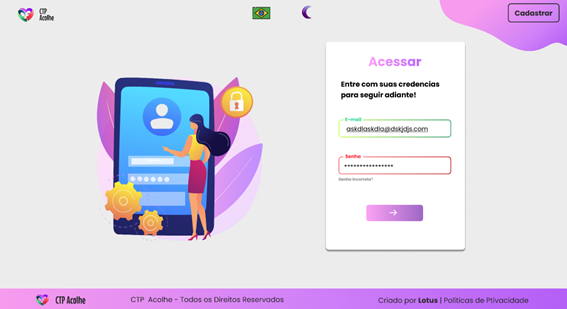
\includegraphics[width=15cm]{prot6.png}
                \caption{Acessar}
                \label{pt}
            \end{figure}
        Observe que ao preencher um campo corretamente, a borda do INPUT ficará verde, 
        \begin{figure}[H]
                \centering
                
\includegraphics[width=15cm]{prot7.png}
                \caption{E-mail}
            \end{figure}
        enquanto quando se é preenchido de maneira incorreta, ficará vermelha.
         \begin{figure}[H]
                \centering
                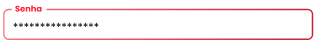
\includegraphics[width=15cm]{prot8.png}
                \caption{Senha}
            \end{figure}
    \newpage
    \item \textbf{Registro de Emoçõe} \\ \\ 
    Após acessar a aplicação, o questionário de registro de emoções é feito ao usuário, na qual ele escolherá 1x por dia, nos dias que acessar, a emoção que mais condiz com o que está sentindo naquele dia. 
          \begin{figure}[H]
                    \centering
                    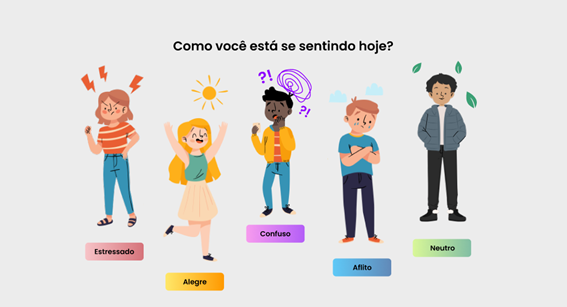
\includegraphics[width=15cm]{prot9.png}
                    \caption{Antes da escolha}
                \end{figure}
            \begin{figure}[H]
                \centering
                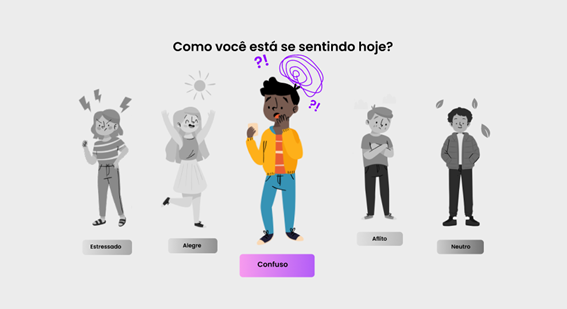
\includegraphics[width=15cm]{prot10.png}
                \caption{Após a escolha}
            \end{figure} 
        Após o registro diário de emoção, o usuário tem acesso livre ao sistema e às demais funcionalidades que ele oferecerá, que estão em desenvolvimento.
        \newpage
    \item \textbf{Usuários sem cadastro} \\ \\
    Para aqueles que ainda não possuem cadastro no sistema, ao clicarem na opção de cadastrar, serão redirecionados para a página de cadastro, na qual poderão preencher os campos com suas informações, a fim de acessar o sistema.
            \begin{figure}[H]
                        \centering
                        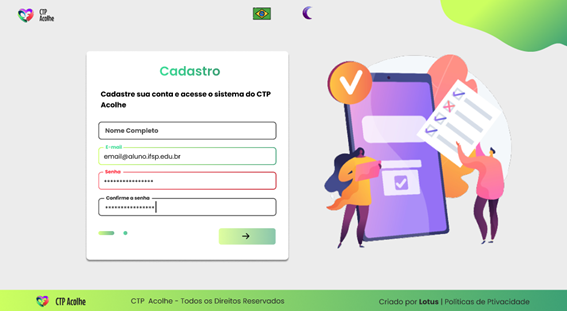
\includegraphics[width=15cm]{prot11.png}
                        \caption{Tela de cadastro}
                    \end{figure}  
        Observe que: \\
        1 - Quando o campo não foi preenchido, aparecerá a descrição dele no centro; 
             \begin{figure}[H]
                            \centering
                            
\includegraphics[width=15cm]{prot12.png}
                            \caption{Nome}
                        \end{figure} 
        2- Quando o campo preenchido for elegível, aparecerá uma borda verde; 
                \begin{figure}[H]
                                \centering
                                
\includegraphics[width=15cm]{prot13.png}
                                \caption{E-mail}
                            \end{figure} 
        3 - Quando as informações não forem aceitas, a borda será vermelha; 
                \begin{figure}[H]
                                \centering
                                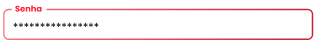
\includegraphics[width=15cm]{prot14.png}
                                \caption{Senha}
                            \end{figure} 
        Enquanto o campo está sendo preenchido, a descrição ficará fixa à parte superior do input.
                 \begin{figure}[H]
                                \centering
                                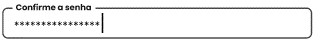
\includegraphics[width=15cm]{prot15.png}
                                \caption{Confirmação de senha}
                            \end{figure}
        Após realizar o cadastro, o usuário poderá acessar o sistema conforme a (Figura~\ref{pt}).
\end{itemize}
    

\end{document}

